%!TEX root = ../dokumentation.tex

\chapter{Implementierung}

\section{Ausgangslage}

\section{Simulation zur Datengenerierung}
Die Simulation erlaubt es eigene Strecken aufbauen.
Dazu gibt es eine High-Level Schnittstelle um verschiedene Streckenabschnitte zusammen zu setzten.
Um eine neue Strecke aufzubauen kann man unterschiedliche Kurven, Kreuzungen und Geraden kombinieren.
Dazu wird die visuelle Darstellung generiert.
Visuelle Darstellung sind Seitenstreifen, Mittelstreifen, Haltelinie und andere Straßenmarkierungen, aber auch Objekte.
Parallel dazu wird die Fahrspur geniert. 
Die Fahrspur ist die Spur in der Mitte der Fahrbahn. 
Das Fahrzeug sollte die Fahrspur möglichst genau entlang fahren, um nicht von der Fahrbahn abzukommen.
Die Fahrspur wird für zwei Anwendungen benötigt:
 - Sie ermöglicht eine Fahrt ohne Fahrzeugsteuerung im AutoDrive Modus
 - Sie ermöglicht eine Evaluierung der Fahrzeugsteuerung. Die Fahrzeugsteuerung wird bewertet, je nach dem wie nah das Fahrzeug an der idealen Fahrspur fährt  

\subsection{Interpolation der Fahrspur}
Das Modul AutomaticDrive kann genutzt werden damit das Fahrzeug entlang der Fahrspur fährt.
Beim Testen dieser Funktion kam es zu einem ruckeligen Fahrverhalten in den Kurven.
Dies liegt an der Speicherung der Fahrspur.
\begin{center}
    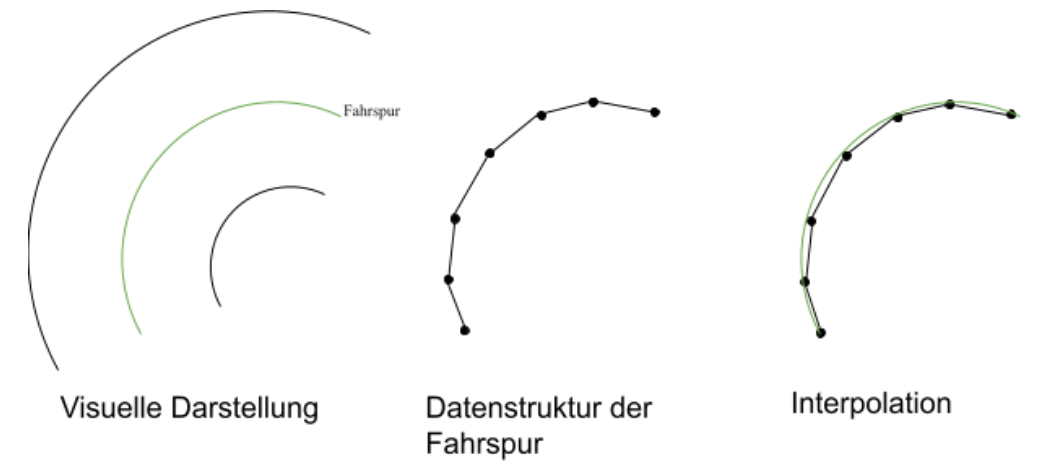
\includegraphics[width=1\textwidth]{Interpolation.png}
\end{center}
Links sieht man die visuelle Darstellung, die generiert wird.
Die Fahrspur (in grün) wird dann gespeichert. 
Dies geschieht indem in einem regelmäsigen Abstand Punkte, die auf der Fahrspur liegen gespeichert werden.
Die Fahrspur wird dann als Liste mit Punkten gespeichert. 
Das AutomaticDrive Modul nutzt dann jeweils die direkte Verbindung von Punkt zu Punkt. 
Dadurch fährt es immer kurz gerade aus, und an jedem Punkt dreht das Fahrzeug auf der Stelle.
Um dieses Verhalten zu verhindern und an die Realität anzupassen wie Interpolation genutzt.
Hier wird Kubische Interpolation genutzt. 
Dabei werden die Punkte nicht mit einer geraden Linie verbunden sondern mit einem Polynom dritten Grades.
Dadurch kann auch die Steigung am Punkt betrachtet werden und es gibt keine Ecken mehr.
Dies zeigt die grüne Linie im dritten Bild.
Die interpolierte Fahrspur stellt nun, mit ausreichender Genauigkeit, mit der originalen Fahrspur im ersten Bild überein.
In Python kann so eine Interpolation zum Beispiel mit der Klasse interp1d aus dem Modul scipy.interpolate berechnet werden.

\subsection{AutoDrive}
Die Positionierung und Orientierung funktioniert mit dem Hinterachsenmittelpunkt H als Basis.
Das Fahrzeug fährt indem der Punkt H mit einer konstanten Geschwindigkeit entlang der Fahrspur fährt.
Die Orientierung des Fahrzeugs ist so definiert, dass das Fahrzeug am Punkt H eine Tangente zur Fahrspur bildet.
Die Tangente kann mit einer Funktioner der Datenstruktur der Fahrspur erechnet werden. 
In einer Kurve kann das Fahrzeug dann so aussehen:

\begin{center}
    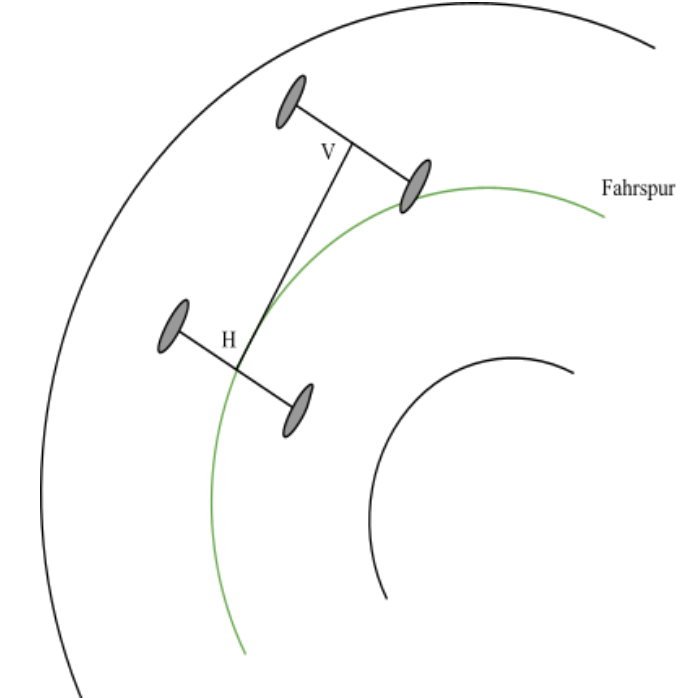
\includegraphics[height=0.5\textwidth]{AutoDrive.png}
\end{center}

Positionierung und Rotation um Punkt H hat sich als realitätsnah erwiesen, da die Kamera, die vorne am Fahrzeug montiert ist, in den Kurven ein ähnliches Bild geliefert hat wie das echte Fahrzeug.


Kamera entlang der Strecke fahren lassen

Um Algorithmen und Model in der Spurerkennung und Situationsklassifizierung zu verifizieren und verbessern, 
benötigt der Auto drive noch eine Möglichkeit den Lenkwinkel auszugeben.
Für den AutomaticDrive nehmen wir ein paralleles Lenksystem an.
Punkt V nach H. $\vec{VH}$ 

Die Vorderräder sind ausgerichtet entlang der Tangente VT am Punkt V zur Fahrspur.
Der Lenkwinkel $\beta$ ist der Winkel zwischen $\vec{VH}$ und $\vec{Lenkrichtung}$. 

\begin{center}
    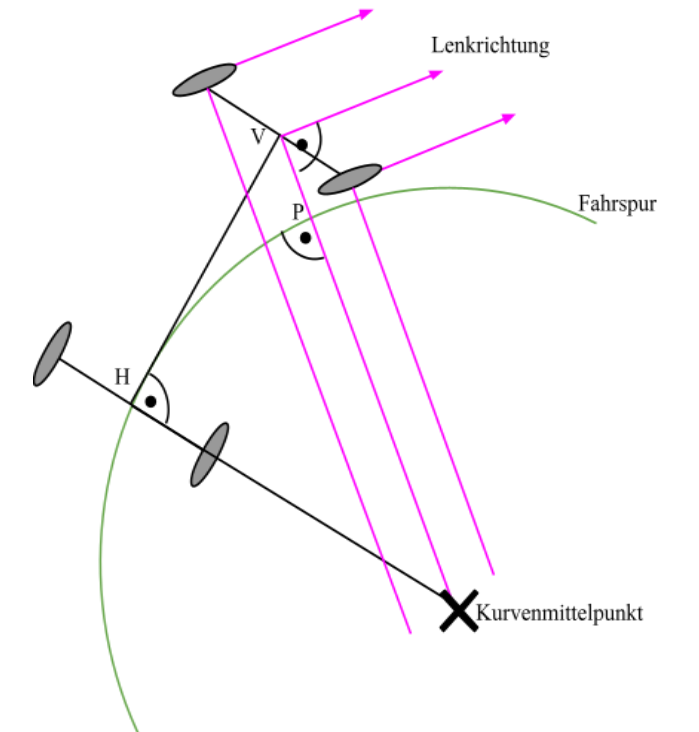
\includegraphics[height=.5\textwidth]{ParallelSteering.png}
\end{center}

PARAMETER INCLUDE AUTODRIVE


\section{Kamera}
Um die Kamera zu simulieren wird camera\_controller plugin genutzt.
Dieses Plugin hat diverse Einstellungsmöglichkeiten für die Kamera wie FoV, clipping, Farbformat, Updaterate\dots
Es verfügt außerdem über fortgeschrittenere Einstellungsmöglichkeiten wie Distortion oder Noise.

Die Auflösung der echten Kamera ist 2456x2054 Pixel, daher wird die virtuelle Kamera ebenfalls auf diese Auflösung eingestellt.

\begin{lstlisting}
<link name="front_camera_link">...</link>
<joint name="front_camera_joint" type="fixed">...</joint>
<gazebo reference="front_camera_link">
    <sensor name="front_camera" type="camera">
        <plugin name="camera_plugin" filename="libgazebo_ros_camera.so">...</plugin>
        <update_rate>25</update_rate>
        <camera>
            <horizontal_fov>2.064911321881509</horizontal_fov>
            <image>
                <width>2456</width>
                <height>2054</height>
                <format>L8</format>
            </image>
            <clip>
                <near>0.1</near>
                <far>4</far>
            </clip>
        </camera>
    </sensor>
</gazebo>
\end{lstlisting}
Die Position und Orientierung der Kamera wird genau ermittelt, um die simulierte Kamera an die selbe Position zu bringen.
Kleine Ungenauigkeiten können schon große negative Auswirkungen haben. 
Die Fahrzeugsteuerung transformiert das Kamerabild ein eine Vogelperspektive um das Bild für die Spurerkennung vorzubereiten.
Die Transformation vom Kamerabild in die Vogelperspektive ist definiert durch die IPM-Matrix.
Um zu überprüfen ob die Kamera gut platziert ist, kann man ein Kamerabild nehmen und es mit der IPM-Matrix transformieren. 
\begin{center}
    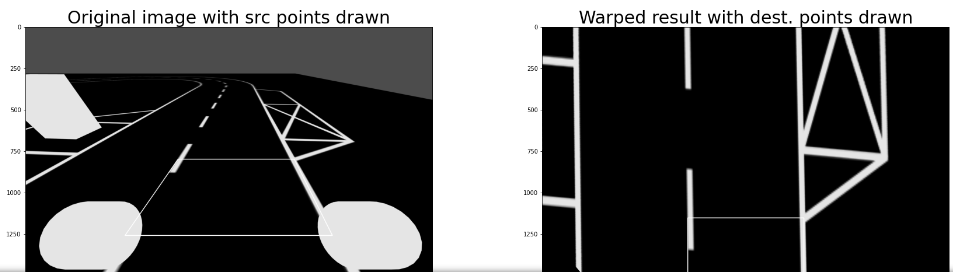
\includegraphics[width=1\textwidth]{ipm.png}
\end{center}
Wenn bei der Transformation ein solches Bild herauskommt, stimmt die Kameraplatzierung mit der IPM-Matrix überein.



\section{statische Fortbewegung}
Der Lenkwinkel muss irgendwie in eine Transformation des Fahrzeugs umgewandelt werden.
Der genaue Lösung wäre eine dynamische Simulation der Räder und Lenkung.
Dies ist ein sehr großer Aufwand und kann viele Probleme bereiten, da es es bei einer dynamischen Simulation sehr viele Variablen gibt.
Mit der statische Fortbewegung versucht man das komplexe Problem auf möglichst einfachem Wege zu lösen. 
Eine Rechnung soll die Transformation möglichst genau abschätzten. 

Für Rechnung sind folgende Parameter gegeben:
\begin{itemize}
    \item[] Lenkwinkel $\alpha$
    \item[] Vorderachsenmittelpunkt V
    \item[] Richtung des Fahrzeugs $\vec{d}$
    \item[] Geschwindigkeit des Fahrzeugs $\vec{v}$
    \item[] deltaTime seit dem letzten Update dt
\end{itemize}

\begin{center}
    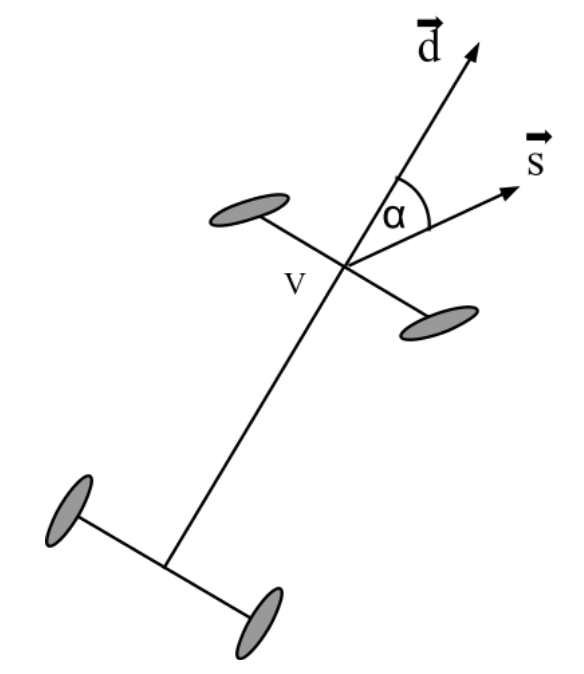
\includegraphics[height=.5\textwidth]{static.png}
\end{center}


Als erstes wird aus dem Lenkwinkel $\alpha$ der Vektor $\vec{s}$ bestimmt.
Außerdem wird die delta Strecke bestimmt. Also die Strecke, die das Fahrzeug seit dem letzten Update gefahren ist.
\[
    ds = dt * |\vec{v}|
\]
Danach wird die neue Position des Vorderachsenmittelpunkts bestimmt. 
Von der alten Position geht man ein bisschen Richtung der Lenkrichtung $/vec{s}$, je nachdem wie viel Zeit vergangen ist oder wie schnell man ist.
\[
    V_{Neu} = V + \vec{s} * ds 
\]
Um die Rotation zu approximieren gibt es eine Konstanten k. k ist abhängig von der Fahrzeuglänge und kann frei gewählt werden.
\[
    dr = k*ds*\alpha
\]
Die neue Orientierung des Fahrzeugs erhält man indem man die neue Rotation dr auf die alte Orientierung addiert.
\[
    \vec{d_{Neu}} = rotate(\vec{d}, dr)
\]

\section{dynamische Fortbewegung}
Die statische Fortbewegung war nur eine Übergangslösung.
Die dynamische Fortbewegung ist genauer. Bisher wurde einfach nur die Position des Fahrzeugs geändert.
Die Physik-Engine, die Gazebo bietet, wird also weder vom AutoDrive noch von der statischen Fortbewegung genutzt.
Ziel der dynamischen Fortbewegung ist es ein Fahrzeug mit vier Rädern zu simulieren.
Das Fahrzeug kann fahren, indem sich die Räder drehen.
Die Hinterräder sollen den Antrieb haben.
Die Vorderräder sollen lenken können.

\subsection*{Vorteile dynamische Fortbewegung}
Wenn für das Fahrzeug, die Massen und die Reibung richtig definiert ist, können bestimmte Fahrverhalten besser abgebildet werden.
Zum Beispiel kann das Fahrzeug dann auch aus Kurven rausgeschläudert werden, wenn es zu schnell ist.
Die zusätzliche Kompläxität, die durch die Räder und das Lenksystem kommt, ist deutlich genauer als die Methode zu statischen Fortbewegung.

\subsection*{URDF Definitionen}
Die Räder des Fahrzeugs werden definiert innerhalb einem Link (siehe urdf unten).
Jeder der vier Links besitzt eine visuelle Komponente und ein Kollisions-Komponente.
Das visuelle Objekt und das Kollisions-Objekt stimmen überein, beide definieren den gleichen Zylinder.
Das Kollisions-Objekt wird benötigt um mit dem Boden zu kollidieren um auf diesem zu fahren.
Jeder physikalisch simulierte Link benötigt einen inertial-Tag.
Dieser definiert die Masse "mass" und die Massenverteilung als inertia Tensor "inertia".

\subsection*{Joints}
Damit sich ein Rad drehen kann, wird es mit einem Joint an dem Fahrzeug befestigt.
Ein Joint ist eine Verbindung zwischen zwei Links. 
In einem Joint wird definiert wie sich die zwei Links zueinander verhalten.
Es gibt die unterschiedliche Typen von Joints:
\begin{itemize}
    \item revolute - Rotiert um eine Achse bis zu gesetzten Ober- und Untergrenze
    \item continous - Rotiert um eine Achse ohne Grenze
    \item prismatic - Gleitet entlang einer Achse bis zu Grenzen
    \item fixed - Dieser Joint verbindet zwei Links fest miteinander. Es gibt keine relative Bewegung
    \item floating - Erlaubt freie Positions- und Rotationsänderung zwischen zwei Links
    \item planar - Erlaubt Bewegung auf einer Ebene
\end{itemize}
\cite{Joint}

\subsection*{Drehen und Lenken}
Die Räder werden alle mit einem Joint mit dem Fahrzeug verbunden.
Der Typ des Joints ist für die Räder continuos. Das bedeuted, dass sich die Räder ohne Einschränkung um eine Achse drehen können.
Die Hinterräder werden direkt mit der Basis des Fahrzeugs verbunden.
Die Vorderräder werden mit einem Zwischenstück verbunden.
Dieses Zwischenstück wird benötigt, da die Vorderräder einen zweiten Joint benötigen um eine Lenkbewegung durchzuführen.
Zwei Links können nur mit einem Joint miteinander verbunden werden.
Vom Mittelstück zur Basis gibt es einen Joint, der die Lenkung möglich macht.
Dieser Joint ist vom Typ revolute. 
Der Joint dreht sich auf der Achse, orthogonal zum Boden.
Er hat Limits bei +-60°.\\
Das Vorderrad kann sich nun um die eigene Radachse drehen, und es kann sich mit dem Mittelstück um die z-Achse drehen.
Der folgende Code definiert das linke Vorderrad "reifen\_front\_links" mit visual, collision und inertial.
Danach wird das Mittelstück "links\_front\_steering" definiert, welches eine einfache Box ist.
Das Mittelstück wird mit der Basis (chassis) verbunden mit einem revolute Joint. 
Das Vorderrad mit mit dem Mittelstück verbunden mit einem continous Joint.
\begin{lstlisting}
<link name="reifen_front_links">
    <visual>
        <origin xyz="0 0 0" rpy="1.57075 0 0"/>
        <geometry>
            <cylinder length ="0.02" radius="0.03"/>
        </geometry>
        <material name="reifenfarbe">
            <color> 1.0 1.0 1.0</color>
        </material>
    </visual>
    <collision>
        <origin xyz="0 0 0" rpy="1.57075 0 0"/>
        <geometry>
            <cylinder length ="0.02" radius="0.03"/>
        </geometry>
    </collision>
    <inertial>
        <inertia ixx="0.0001" ixy="0" ixz="0" iyx="0" iyy="0.0001" iyz="0" izx="0" izy="0" izz="0.0001"/>
        <mass value="0.05"/>
    </inertial>
</link>
<link name="links_front_steering">
    <visual>
        <origin rpy="0 0 0" xyz="0 0 0"/>
        <geometry>
            <box size =".01 .001 .01"/>
        </geometry>
    </visual>
    <inertial>
        <inertia ixx="0" ixy="0" ixz="0" iyx="0" iyy="0" iyz="0" izx="0" izy="0" izz="0"/>
        <mass value="0.01"/>
    </inertial>
</link>
<joint name="basis_zu_links_front_steering" type="revolute">
    <parent link="chassis"/>
    <child link="links_front_steering"/>
    <origin xyz="0.1 0.06 0.03" rpy="0 0 0"/>
    <axis xyz="0 0 1"/>
    <limit lower="-1.1" upper="1.1" effort="10" velocity="100"/>
</joint>
<joint name="links_front_steering_to_reifen_front_links" type="continuous">
    <parent link="links_front_steering"/>
    <child link="reifen_front_links"/>
    <origin xyz="0.0 0.02 0.0"/>
    <axis   xyz="0 1 0"/>
</joint>
\end{lstlisting}
Dieser Code produziert das:
\begin{center}
    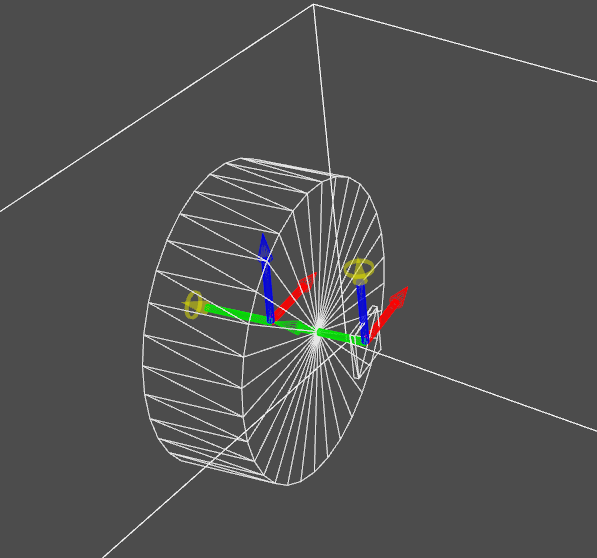
\includegraphics[height=.5\textwidth]{LeftWheel.png}
\end{center}
Hier ist das Linke Vorderrad zu sehen und das dazugehörige Mittelstück.
Man erkennt die Zwei Joints, welche jeweils Rotation um eine Achse erlauben. 

\subsection*{Actuator und Transmissions}
Um die Räder und die Länkung zu steuern, benötigt es einen Motor. 
Für urdf gibt es hierfür Actuator und Transmissions.
Eine Transmission verbindet einen Actuator mit einem Joint. 
Der Actuator, zu Deutsch "Antrieb", gibt eine Bewegung über die Transmission an den Joint weiter.
In diesem Fall ist es eine Drehbewegung, da nur revolute und continous Joints genutzt werden.
Der Actuator definiert das Hardware Interface.
Bei den Hinterradantrieben wird ein Velocity Interface genutzt, da die zu steuernde Größe die Geschwindigkeit des Rads, bzw. des Joints ist.
Für die Vorderradlenkung wird ein Effort Interface genutzt, da die zu steuernde Größe der Winkel des Rads ist.
Außerdem kann der Actuator eine machanische Reduktion der Drehgeschwindigkeit definieren.
Die Definition einer Transmission mit Actuator sieht so aus: 
\begin{lstlisting}
<transmission name="transmission_front_left_wheel">
    <type>transmission_interface/SimpleTransmission</type>
    <joint name="basis_zu_links_front_steering">
        <hardwareInterface>hardware_interface/EffortJointInterface</hardwareInterface>
    </joint>
    <actuator name="motor_front_left_wheel">
        <hardwareInterface>hardware_interface/EffortJointInterface</hardwareInterface>
        <mechanicalReduction>1</mechanicalReduction>
    </actuator>
</transmission>
\end{lstlisting}

\subsection*{Controller}
Um die Actuator zu steuern kann man das Package ros\_control nutzten.
Dies bietet eine Reihe verschiedener Controller.
Controller können einen Actuator nach PID-Steuerung steuern.
Um die Controller zu benutzen wird ein neues Package erstellt.
Das Package $/simulation/src/gazebo\_controller$ beinhaltet eine Launchdatei und eine Parameterdatei.
Die Parameterdatei definiert die vier verschiedenen Controller.
Zwei für den Hinterradantrieb und zwei für die Vorderlenkung.
Die Controller für den Antrieb sind JointVelocityController, die Controller für die Lenkung sind JointPositionController.
Von dem Antrieb soll die Geschwindigkeit gesteuert werden, von der Lenkung soll die Position bzw. die Rotation gesteuert werden.
In der Parameterdatei werden auch die zugehörigen Joints und die PID Parameter definiert.
Die Launchdatei nutzt die Parameterdatei und lädt damit die Controller über einen controller\_spawner.
Die Launchdatei wird in der master.launch-Datei wie folgt aufgerufen:
\begin{lstlisting}
<include if="\$(eval include_automatic_drive == false)" file="\$(find gazebo_controller)/launch/robot_control.launch"></include>
\end{lstlisting}
Die Controller werden nur initialisiert, wenn AutomaticDrive nicht genutzt wird.

\subsection{PID Regelung}
PID Regler werden eingesetzt um eine bestimmte Regelgröße zu regeln. 
Der Regler vergleicht den Soll- und Istwert der Regelgröße und versucht deren Differenz zu minimieren.
Dieses Ziel verfolgt er über drei Komponenten: 
Die Proportional-Komponente, welche abhängig von der aktuellen Differenz zwischen Ist- und Sollwert ist.
Die Integral-Komponente, welche abhängig von der vergangenen Differenz zwischen Ist- und Sollwert ist.
Die Differentail-Komponente, welche abhängig von der zukünftigen Differenz zwischen Ist- und Sollwert ist.
Wie groß der Einfluss der jeweiligen Komponente ist lässt sich über die Parameter P,I und D steuern.
\cite{PIDRegler:2020}

Alle vier Controller benötigen angepasste PID-Parameter.
Schauen wir uns zuerst die Vorderradlenkung an. 
Dafür wird die Simulation mit der Fahrzeugsteuerung verbunden.
Aus der Fahrzeugsteuerung werden nun Lenkwinkel an die Simulation geschickt.
Dieser Lenkwinkel ist der Sollwert, und wird durch die rote Linie im Diagram dargestellt.
\begin{center}
    \includegraphics[height=.5\textwidth]{Türkis15-2-5Pink15-0-0.png}
\end{center}
Auf diesen Sollwert hören zwei Controller.
Der Controller für das linke Rad hat eine PID-Einstellung von 15-0-0.
Sein Istwert ist durch die pinke Linie im Diagram dargestellt.
Der Controller für das rechte Rad hat eine PID-Einstellung von 15-2-5.
Sein Istwert ist durch die türkisene Linie im Diagram dargestellt.\\
Bis ca. t = 144 ist der pinkene Controller ein wenig näher am Sollwert als der Türkisene.
Aber ab t = 144.5 überkorrigiert sich der pinke Controller ständig. 
Im Gegensatzt dazu ist der türkisene Controller ab t = 144.5 näher am Sollwert, da er nicht überkorrigiert.
Der türkisene Controller hat einen D-Wert von 5. Dadurch überkorrigiert er nicht ständig sonder berührt die Sollwert Kurve eher.\\
Durch so Tests können PID-Parameter optimiert werden, sowohl für die Lenkung als auch für den Antrieb des Fahrzeugs.

\subsection{Ackerman Lenkung}
Ziel der Simulation ist es bei gegebenem Lenkwinkel und Geschwindigkeit das Fahrzeug entsprechend zu bewegen.
Die Geschwindigkeit wird an die zwei Geschwindigkeitscontroller gegeben.
Der Lenkwinkel wird an die zwei Lenkcontroller gegeben.
Hierbei treten jedoch zwei Probleme auf:

Wenn sich beide Hinterräder in der genau gleichen Geschwindigkeit drehen, kann es zu Problemen in Kurven kommen.
Das äußere Rad muss eine längere Strecke in der gleichen Zeit wie das innere Rad fahren. 
Dadurch kann es zu ungewünschten Kräften und Rutschen kommen.
Im echten Fahrzeug wird dieses Problem durch ein Differentialgetriebe gelöst.
In der Simulation hat sich das als kein großes Problem erwiesen und es bleibt erstmal bei zwei Controllern mit der genau gleichen Geschwindigkeit, auch in den Kurven.

Das zweite Problem ist die Lenkung. 
Wenn man den Lenkwinkel direkt an beide Controller weitergibt hat man eine Parallellenkung.
Das Fahrzeug mit Parallellenkung sieht in einer Kurve so aus:  
\begin{center}
    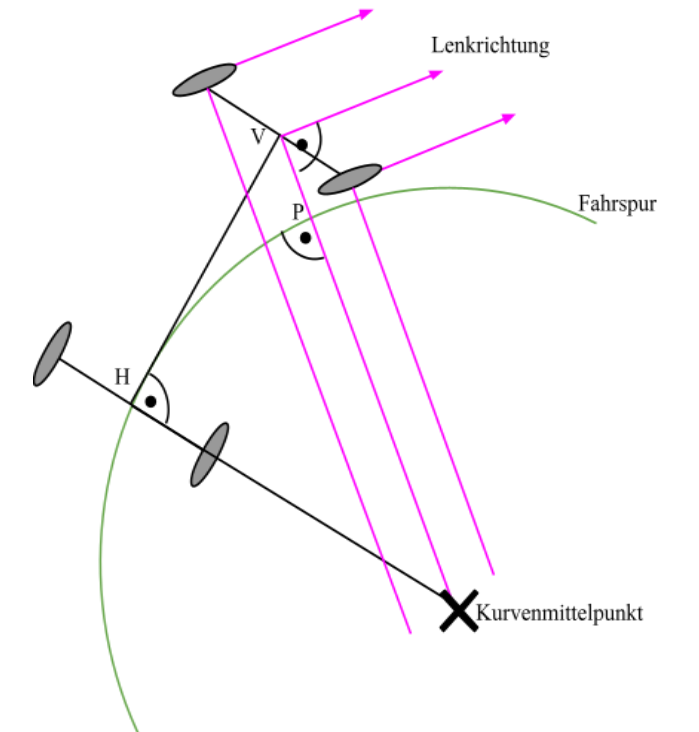
\includegraphics[height=.5\textwidth]{ParallelSteering.png}
\end{center}
Das Fahrzeug fährt um den Kurvenmittelpunkt herum. 
Wenn ein Rad eine Kurve fährt, ist es so ausgerichtet, dass es entlang einer Tangenten auf dem Kreis um den Kurvenmittelpunkt fährt.
Die Hinterräder des Fahrzeugs fahren um den Kurvenmittelpunkt.
Die Vorderräder sind allerdings nicht entlang eines Kreises um den Kurvenmittelpunkt orientiert sondern parallel zur Lenkrichtung.
Die Lenkrichtung geht aus vom Vorderachsenmittelpunkt V.
Dies kann ebenfalls zu Rutschen und ungewollten Kräften auf Räder und Lenkung führen.
Um das zu verhindern wird im echten Fahrzeug eine Ackermann-Lenkung verwendet. 
Diese sieht in einer Kurve so aus:
\begin{center}
    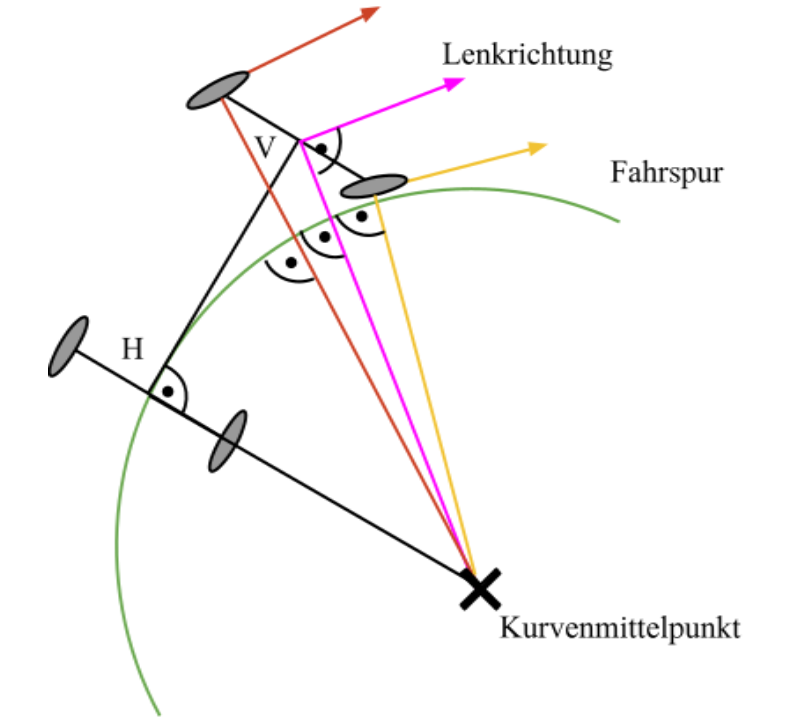
\includegraphics[height=.5\textwidth]{Ackermann.png}
\end{center}
Im Gegensatz zu Parallellenkung sind nun auch die Vorderräder entlang einem Kreis um den Kurvenmittelpunkt ausgerichtet.
Das linke Rad hat nun einen anderen Winkel wie das rechte Rad.

Wie die Ackerman-Lenkung, per Hardware, im echten Fahrzeug umgesetzt ist hier unwichtig.
Um die Ackerman-Lenkung zu simulieren, können aus einem gegebenen Lenkwinkel, jeweils der Winkel für das rechte und linke Rad berechnet werden.

\begin{center}
    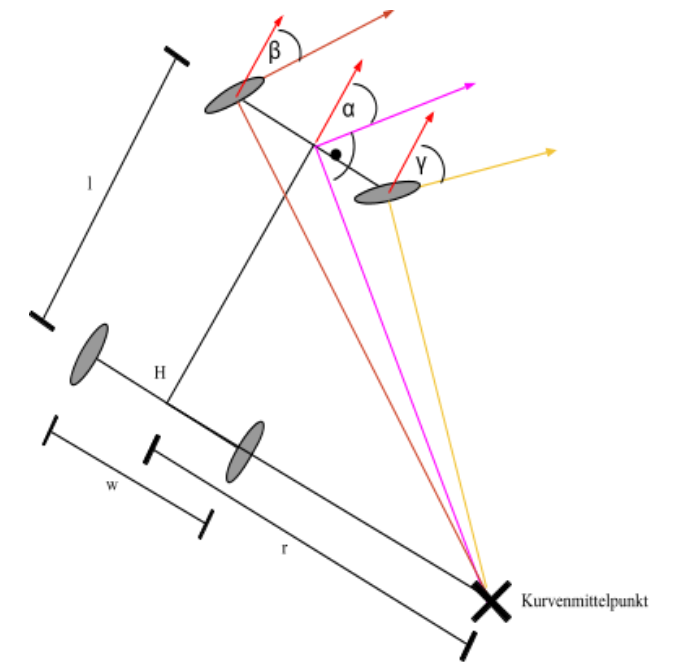
\includegraphics[height=.5\textwidth]{AckermannBerechnung.png}
\end{center}

Ziel ist es die Winkel $\beta$ und $\gamma$ zu bestimmen.
Gegeben ist der Lenkwinkel am Vorderachsenmittelpunkt $\alpha$. 
Mit der Fahrtrichtung und $\alpha$ lässt sich die pinke Linie konstruieren. 
Außerdem ist gegeben dass die Hinterachse auf einer Geraden mit dem Kurvenmittelpunkt liegt.
Der Schnittpunkt der pinken Linie und dieser Geraden ist der Kurvenmittelpunkt.
Die Strecke von H zum Kurvenmittelpunkt wird definiert als r.
Die Strecke w ist der Radabstand zwischen den rechten und linken Rädern.
Die Strecke l ist der Radabstand zwischen den vorderen und hinteren Rädern.
Aus der Pinken Strecke und den Strecken r und l bildet sich ein Dreieck mit rechtem Winkel bei H.
Daraus folgt 
\begin{equation} \label{eq:1}
    \tan(\alpha) = \frac{l}{r}
\end{equation}
Wenn man den Punkt H um $\frac{w}{2}$ nach rechts und links verschiebt kann man zwei weitere rechtwinklige Dreiecke konstruieren.
Diese beinhalten jeweils die braune oder gelbe Strecke. 
Aus den zwei Dreiecken gehen folgende Gleichungen hervor:
\begin{equation} \label{eq:2}
    \tan(\beta) = \frac{l}{r-w/2} 
\end{equation}
\begin{equation}  \label{eq:3}
    \tan(\gamma) = \frac{l}{r+w/2} 
\end{equation}
Umformung Gleichung \ref{eq:1}
\begin{equation} \label{eq:4}
    r = \frac{l}{\tan(\alpha)}
\end{equation}
Setzte man Gleichung \ref{eq:4} in Gleichung \ref{eq:2} ein so erhält man
\[ \tan(\beta) = \frac{l}{\frac{l}{\tan(\alpha)}-w/2}\] 
\[ \iff \beta = \arctan(\frac{l}{\frac{l}{\tan(\alpha)}-w/2})\] 
Analog dazu erhält man die Gleichung für $\gamma$
\[ \gamma = \arctan(\frac{l}{\frac{l}{\tan(\alpha)}+w/2})\] 
Mit diesen zwei Gleichungen lassen sich die Winkel $\beta$ und $\gamma$ bestimmen.
Die Radabstände l und w sind fest in der Simulation definiert.
Beide individuelle Lenkwinkel $\beta$ und $\gamma$ sind nur von einer Variablen abhängig: Dem Lenkwinkel am Vorderachsenmittelpunkt $\alpha$.
\cite{ackerman:2021}